% Figure for the

\begin{figure}
\center

	\begin{subfigure}[b]{0.4\textwidth}
	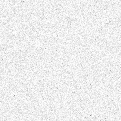
\includegraphics[width=\linewidth]{images/findings/round1/flipbook_a.png}
	\caption{Starting Weights}
	\end{subfigure}
	~
	\begin{subfigure}[b]{0.4\textwidth}
	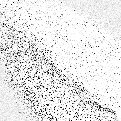
\includegraphics[width=\linewidth]{images/findings/round1/flipbook_b.png}
	\caption{After 200,000 games played}
	\end{subfigure}

	\begin{subfigure}[b]{0.4\textwidth}
	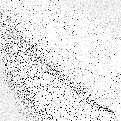
\includegraphics[width=\linewidth]{images/findings/round1/flipbook_c.png}
	\caption{After 400,000 games played}
	\end{subfigure}
	~
	\begin{subfigure}[b]{0.4\textwidth}
	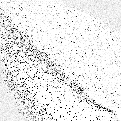
\includegraphics[width=\linewidth]{images/findings/round1/flipbook_d.png}
	\caption{After 600,000 games played}
	\end{subfigure}

	\begin{subfigure}[b]{0.4\textwidth}
	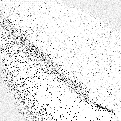
\includegraphics[width=\linewidth]{images/findings/round1/flipbook_e.png}
	\caption{After 800,000 games played}
	\end{subfigure}
	~
	\begin{subfigure}[b]{0.4\textwidth}
	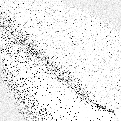
\includegraphics[width=\linewidth]{images/findings/round1/flipbook_f.png}
	\caption{Final Weights}
	\end{subfigure}

\caption{%
	Training weights representation for Agent 0's \texttt{hand\_max\_avg}
	strategy when the agent is the dealer
	over the course of the one million games of Round 1.%
}
% TODO: figure out axes
\label{fig:r1-flip}
\end{figure}
